
The pteropod IBM is structured in two modules, a population module, and a physical module. The population module simulates a simplified life cycle of shelled pteropods parameterized using compiled published experimental data on pteropod life history, behavioral, physiological and morphological traits. The physical module computes the movement (i.e. advection and DVM) of the pteropods, and keeps track of the environmental conditions that the pteropods experience each day. The processes that we simulate in this model are visualized in figure \ref{fig:model_visualization}. In the following sections we present the physiological, life history, behavioral, and morphological traits considered in our IBM.



\begin{figure*}[tbh!]
    \centering
    
        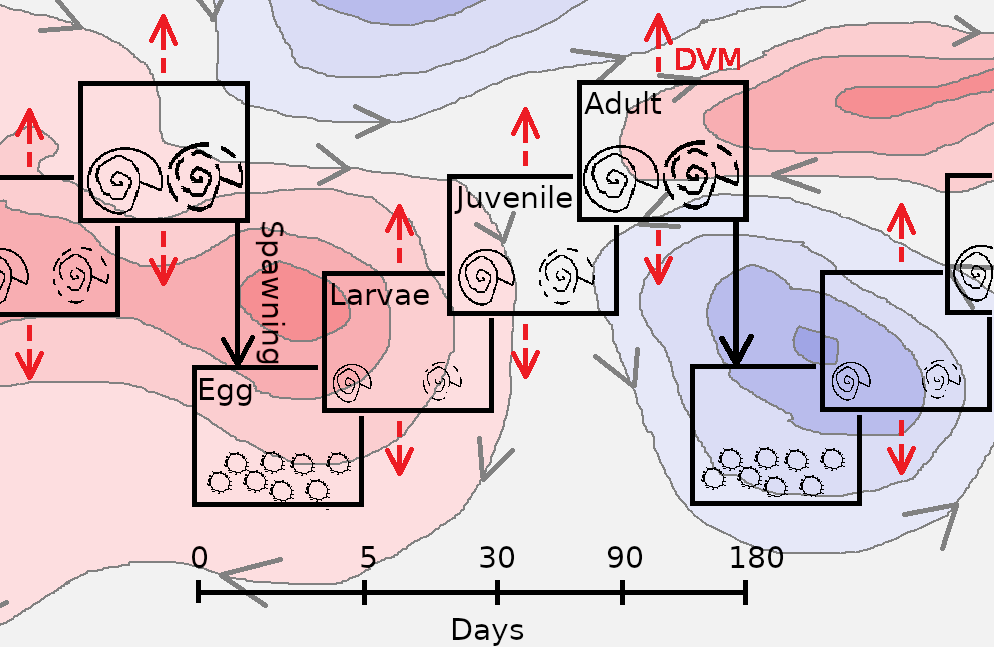
\includegraphics[scale=0.5]{images/model_visualization_sketch_with_circulation.png}
       
    
    \caption{Visualization of the processes included in the pteropod IBM model. In the front are the four stages (egg, larvae, juvenile, and adult) included in the population module shown by the boxes. The duration of each stage is given in number of days after hatching. The spawning events are marked by the black downward arrows. Stages performing diurnal vertical migration (DVM) are shown with the red arrows, and stages affected by dissolution by the shells with gaps. The background represents the ocean circulation, and environmental conditions that the modeled pteropods experience.}
    \label{fig:model_visualization}
\end{figure*}

\subsection{Physiological traits} \label{sec:physiological_traits}
The physiological traits simulated in the population model are the longevity, and growth rate. We use the longevity of temperate pteropod species as a basis for modeling the longevity of pteropods, due to the decreased influence of seasonal changes in environmental factors \citep[e.g. temperature and food availability; ][]{Bednarsek2012PteropodDistribution,Wang2017Lifecycle} on pteropod growth and longevity compared to polar species \citep{Manno2017ReviewPteropodVulnerability}. Under laboratory conditions the longevity of temperate \textit{Limacina retroversa} individuals was observed to be around six months \citep{Thabet2015Lifestages}. A similarly long longevity of six months is observed on the population level for \textit{L. helicina} during optimal growth conditions in spring in the temperate North Pacific \citep{Wang2017Lifecycle}. Thus, the pteropods in our IBM have a basis longevity of six months.

The growth rates of shelled pteropods are taken from the three-year cohort analysis of the \textit{L. helicina} populations in the temperate North Pacific \citep{Wang2017Lifecycle}. \cite{Wang2017Lifecycle} provide the shell length ($L$) of pteropods as a function of time using measured length-frequency observations and a variation of the \textit{von Bertalanffy growth function} \citep[VBGF; ][]{Bertalanffy1938}, which considers seasonal changes ($S$) in growth rates. The formula used is as follows \citep{Somers1988,Wang2017Lifecycle}:
\begin{eqnarray}
L(t) & = & L_{\infty} \cdot (1 - e^{(K(t-t_0) + S(t) - S(t0))}), \\
S(t) & = & \frac{CK}{2\pi} \cdot sin(2\pi (t-t_s)), \\
t_s + 0.5 & = & WP,
\end{eqnarray}
\noindent
where $L(t)$ denotes the length at age $t$, $L_{\infty}$ the maximum length, $K$ how fast $L_{\infty}$ is reached, $C$ the amplitude of growth oscillations, $t_0$ the age at $L=0$, $t_s$ the time between $t=0$ and the onset of oscillations in growth, and $WP$ the fraction of the year where growth is at its slowest. As was the case for the longevity, we use the growth function for the spring population as the basis growth function for our IBM (Fig. \ref{fig:optimal_growth}), where the values for $WP=0.1$ and $C=0.4$ where taken from \cite{Wang2017Lifecycle}. The values for $K=5.07\, s^{-1}$ and $L_{\infty} = 4.53\, mm$ are average values reported in \cite{Wang2017Lifecycle}.


\begin{figure*}[tbh!]
    \centering
    
        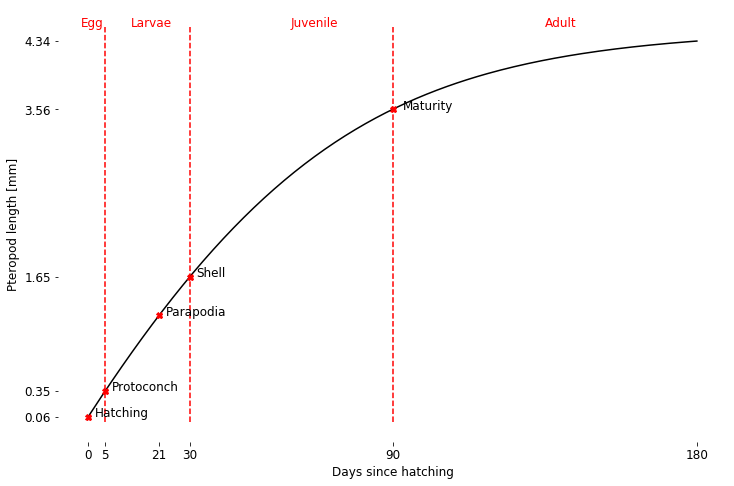
\includegraphics[scale=0.5]{images/Optimal_growth.png}
       
    
    \caption{Pteropod length growth (black line) calculated based on the growth rates described in \cite{Wang2017Lifecycle}. The x-axis denotes the days since hatching. The y-axis denotes the length of the pteropod in mm. The red vertical lines separate the growth rate into the life stages, egg, larvae, juvenile, and adult. The red dots mark the hatching at day 0, and the development of key traits such as the protoconch (larval shell; day 5), parapodia (wings; day 21), shell (day 30), and maturity (day 90).}
    \label{fig:optimal_growth}
\end{figure*}


\subsection{Life history traits}\label{sec:life_history_traits}

Shelled pteropods have shown a  life stage specific sensitivity to changes in environmental condition \citep{Thabet2015Lifestages,Bednarsek2016CumulativeEffects}. Thus, the shell growth rate described above was divided into four life stages in our IBM, i.e. into the egg, larvae, juvenile, and adult stage. These four stages aggregate the ten-stage life cycle of the temperate pteropod \textit{Limacina retroversa} \citep{Howes2014Lab,Thabet2015Lifestages}. The transition between the stages is defined based on the timings of key traits such as the development of wings (parapodia), larval shell (protoconch), juvenile and adult shell, and maturity, since the aim of this study is to characterize the effects of acidification throughout the life of shelled pteropods that perform DVM. Thus, in combination with the shell growth rate described in the section \ref{sec:physiological_traits}, we define the size a pteropod needs to reach to transition between one stage to the next (Fig. \ref{fig:optimal_growth}).


The egg stage lasts for five days. The egg stage summarizes all stages between spawning up to (but not including) the development of the protoconch \citep{Thabet2015Lifestages}. The larvae stage lasts for 25 days. This stage starts with the development of the protoconch, and includes the development of parapodia after roughly three weeks from spawning \citep{Thabet2015Lifestages}. The juvenile stage lasts for 60 days. This stage corresponds to the stage of rapid shell growth \citep{Thabet2015Lifestages}. Finally, the adult stage lasts for 90 days, and corresponds to the reproductive stage where pteropods develop female gonads \cite{lalli1989pelagic,Thabet2015Lifestages,Bednarsek2016CumulativeEffects}.


The eggs of epipelagic shelled pteropod species are spawned as buoyant free-floating masses at the surface \citep{Lalli1978Reproduction,Paranjape1968egg,Schalk1990SeasonalSpatial,Gannefors2005Overwintering,Comeau2010Predation,Manno2016EggsAcidification}. While there is evidence for continuous low level spawning  throughout the year \citep{Wang2017Lifecycle,Thabet2015Lifestages}, pteropod  adults in a population have been found to have phases of synchronized widespread spawningm \citep[e.g. in spring and autumn][]{lalli1989pelagic,Thabet2015Lifestages,Wang2017Lifecycle}. During main spawning phases a pause of roughly 20 days has been observed between spawning of eggs \citep{Paranjape1968egg}. We modeled the time between spawning by defining a Egg Release Readiness Index (ERR), which is set to a random number between zero and one at maturation, increases by $\frac{1}{20}$ each day, and upon reaching $ERR \geq 1.0$ the eggs are released, and ERR is set to zero \citep[similar to the Clutch Readines Fraction presented in ][]{Miller1998CalanusIBM}.
% After the main spawning events adult pteropods have been observed to die \citep{Dadon1992Reproduction,Gannefors2005Overwintering,Hunt2008TopPredators,Howes2014Lab}.
% Resting stages



\subsection{Morphological traits}

In the previous section \ref{sec:life_history_traits}, we presented the duration of the four stages used in our IBM. The combination of the stage duration with the length growth presented in section \ref{sec:physiological_traits} allows us to define the size required for each individual to develop into the next stage. Under optimal or spring conditions, the egg, larvae, and juvenile stages last until they reach $0.35\,mm$, $1.65\, mm$, and $3.56\, mm$, respectively (Fig. \ref{fig:optimal_growth}). 

The stages of our IBM were defined based on the developmental timings of specific traits, such as the protoconch, and juvenile and adult shell (section \ref{sec:life_history_traits}). Both types of shells are susceptible to acidification with differing sensitivity \citep{Bednarsek2017ApplicationPteropodShell,Thabet2015Lifestages}. Such a definition allows us to characterize the calcification and dissolution rates for each pteropod at different stages of their life. To this end, we defined the calcification and dissolution rates as a function of the aragonite saturation state ($\Omega_{arag}$), as well as their shell length, were dissolution and calcification starts at the larvae stage.


\textbf{Tons of equations here}

The final morphological trait we model in our IBM are the number of eggs produced by each individual. Upon reaching maturity, pteropod adults begin spawning eggs \citep{lalli1989pelagic,Gannefors2005Overwintering}. The number of eggs produced per reproductive pteropod adults has a high variability, ranging between $524$ and $10'051$ eggs (mean $5'936$) per \textit{L. helicina} female, and between $83$ and $650$ eggs (mean $260$) per \textit{L. retroversa} in a $20$ day period \citep{Lalli1978Reproduction}. This high variability in number of eggs is likely linked to the environmental conditions that pteropods experience \citep{Manno2016EggsAcidification}, since for instance reproductive \textit{L. helicina} adults produce between $465$ and $708$ eggs (mean $565$) over the 20 day period \citep{Paranjape1968egg}. As was the case for the physiological traits (section \ref{sec:physiological_traits}) we use the estimates for the warmer regions for our IBM, i.e. reproductive adults spawn $565$ eggs.



\subsection{Behavioral traits}

\textbf{Paragraph on motility, i.e. upward, downward swimming speed}

\textbf{Paragraph on DVM, i.e. maximum depth, and timing}





% \subsection{Physiological traits}
% The physiological traits simulated in the population model are the longevity, growth rate, and starvation tolerance of pteropods.

% The longevity and description of life stages for individual pterpods has been found to be around six months under laboratory conditions \citep[\textit{L. retroversa}; ][]{Thabet2015Lifestages}. This longevity of approximately six months for pteropods agrees with new findings on the longevity  of approximately six months in spring and eleven months for overwintering populations of \textit{L. helicina} observed in the temperate North Pacific \citep{Wang2017Lifecycle}.
% The longevity of six months for individual pteropods represents a longevity under optimal conditions. Thus, we used the population level longevity \citep[six and eleven months][]{Wang2017Lifecycle} to infer the longevity of individuals in our model. 

% The growth rate of shelled pteropods has been relatively uncertain \citep{Manno2017ReviewPteropodVulnerability}. However, the cohort analysis by \cite{Wang2017Lifecycle} revealed a strong seasonality, and dependence of the growth rate on temperature. The cohort analysis identifies an overwintering stage \citep{Wang2017Lifecycle}, which confirms previous observations of a veliger stage that overwinters before transitioning to a juvenile stage \citep{Paranjape1968egg,Gannefors2005Overwintering,Hunt2008TopPredators}, and thus extends the longevity of the pteropods to approximately eleven months in the temperate North Pacific. 


% The shell growth function uses a variation of the \textit{von Bertalanffy growth function} (VBGF), which considers seasonal changes in growth rates \citep{Somers1988,Wang2017Lifecycle}.


% \begin{itemize}
%     \item Maximum growth rate (Wang)
%     \item starvation tolerance (egg production despite starvation?) (search for this reference)
%     \item longevity (variable but some studies found around 6 months/11 months)(Wang, thabet, bednarsek)
% \end{itemize}

% \subsection{Life history traits}
% \begin{itemize}
%     \item Sexual reproduction
%     \item Reproduction frequency (Peranjape, clutch readiness)
%     \item Size at maturation (Wang)
%     \item resting stages (overwintering?) (Wang)
% \end{itemize}









\subsection{physical module}




(Check files to see the population drift at 31.Dec compared to initial population.

\textbf{
Need to read up on unbeaching functions used and reseeding approaches (Plankton zoonation problem!!). Also re-running population appears to have some problems on the main code! (does not compile, and dealing with no exposure does not work with the current implementations)}



Subject of each section:
\begin{itemize}
    \item Description of pteropod IBM
        \begin{itemize}
            \item One subsection per module (population and particle module) \citep{Erguler2018Modules}
            \item Description of the DVM kernel as a function of size \citep{Bianchi2013ImportanceDVM,Bednarsek2015VerticalDistribution,Murphy2016UpwardSwimming,Chang2012SwimmingSpeedSize,Byrne1984SettlingSpeed,Bergan2017SwimmingSinkingSpeeds}
            \item Description of unbeaching function \citep{Delandmeter2019Unbeaching}
            \item Description of exposure tracker \citep{Bednarsek2017ExposureHistory}
            \item Description of growth function \citep{Wang2017Lifecycle,Somers1988}
            \item Description of chosen life-stages \citep{Thabet2015Lifestages,Howes2014Lab}
            \item Description of mortality \citep{Bednarsek2016CumulativeEffects}
            \item Description of fecundity and clutch readiness \citep{Paranjape1968egg,Manno2016EggsAcidification,Bednarsek2016CumulativeEffects}
            \item Description of dissolution and repair functions, and pteropod weight changes \citep{Bednarsek2014CalcificationDissolution,Comeau2010RepairRates}
            \item Problems with the model (e.g. drift from coast, re-seeding approaches, 
        \end{itemize}
    \item Description of model tuning to the timing of abundance peaks as done for other IBMs \citep[e.g. ][]{Miller1998CalanusIBM}, and vertical distribution
    \item Description of ROMS hindcast simulation and using the CalCS as a case study
    \item Model validation
    
    
    \item Case study of the effect of acidification on shelled pteropods.
    \begin{itemize}
        \item Description of approach to separate between the effect of DVM, and life-stages in relation to acidification (i.e. advection-only model, no-DVM model, no-life-stages model, and full model)
        
        \item Description of exposure metrics (e.g. average shell size, CaCO$_3$ content, timing of abundance peaks individuals reaching maturity, deviation from optimal growth function, amount of dissolved CaCO$_3$)
    \end{itemize}
    
    
\end{itemize}